\chapter{Algorithm and Data Structures of Sparse Triangular Solve}
% \section{Algorithm and Data Structures of the Forward/Backward Substitution}

\label{sec:algo}

Let $A$ be an $N \times N$ matrix and $x$ and $b$ be vectors of size $N$.
The linear system $A x = b$ is solved via $LDL^T$ decomposition by factorizing $A$
into a lower diagonal matrix $L$ and a diagonal matrix $D$ 
such
that $A =
LDL^T$.
The system is then solved in three steps. First,
$
  \label{eq:fw}
  Ly=b
$
is solved via forward substitution. This is followed by a diagonal solve
$
  \label{eq:dg}
  Dz=y,
$
and afterwards the resulting $z$ vector is used to solve for the solution vector 
%
$
  \label{eq:bw}
  L^Tx=z
$
% 
% via backward substitution. In sparse solver packages, such as, e.g.,
% PARDISO~\cite{schenk-2004}, 
via backward substitution. In 
PARDISO, 
the forward substitution is performed columnwise, starting with the
first column.
%mw first column, as depicted in Fig.~\ref{algo:triangular}~(a).
The data dependencies here allow us to store vectors $y$, $z$, $b$, and $x$ in
only one vector $r$. 
When column $j$ is reached, $r_j$ contains the solution for $y_j$. 
All other elements of $L$ in this column, i.e.,\ $L_{ij}$ with $i = j + 1,
\ldots, N$, are used to update the remaining entries in $r$ by 
%
\be
  r_i = r_i - r_j L_{ij}.
  \label{eq:algo:fw:pardiso}
\ee
%
The backward substitution with~$L^T$ would take place rowwise, but PARDISO
uses $L$ and performs the substitution columnwise.
In contrast to the forward substitution , the
%mw uses $L$ and performs the substitution columnwise, as shown in 
%mw Fig.~\ref{algo:triangular}~(b).  In contrast to the forward substitution, the
iteration over the columns starts at the last column $N$ and proceeds to
the first one.  
If column $j$ is reached, then $r_j$, which contains the $j$-component of the
solution vector $x_j$, is computed by subtracting the dot product of the
remaining elements in the column $L_{ij}$ and the corresponding elements of
$r_i$ with $i = j + 1, \ldots, N$ from it:
%
\be
  r_j = r_j - r_i L_{ij} .
  \label{eq:algo:bw:pardiso}
\ee
%
After all columns have been processed $r$ contains the 
desired
solution of $x$.

%\begin{figure}[t]
%  \centering
%    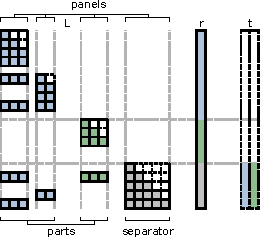
\includegraphics[width=0.55\linewidth,clip=true]{images/parts-panels-separator}
%  \caption{Sparse matrix data structures in PARDISO. Adjacent columns of $L$ exhibiting the same
%structure form panels also known as supernodes.
%Groups of panels which touch independent elements of the right-hand side $r$ are
%parts. The last part in the lower triangular matrix $L$ is called the separator.}
%  \label{fig:algo:ds}
%\end{figure}

The sparse matrix is stored in a PARDISO specific format shown in
Figure~\ref{fig:algo:ds}.
Adjacent columns exhibiting the same row sparsity structure form a
\textit{panel}, also known as a \textit{supernode}.
A panel's column count is called the \textit{panel size} $\panelsize$.
The columns of a panel are stored consecutively in memory excluding the zero
entries. 
Note that columns of panels are padded in the front with zeros so they get the 
same length as the first column inside their panel. 
The padding is of utmost performance for the PARDISO solver to use Level-2/3
BLAS and LAPACK functionalities. Please see~\cite{20.500.11850/144477} for more
details.
Furthermore, panels are stored consecutively in the \vlnz{} array. 
Row and column information is now stored in accompanying arrays.
%2 The \texttt{xsuper} array stores for each panel the index of its first column. 
%Also note that here column indices are the running count of nonzero columns.
Column indices are used as indices into the \vxlnz{} array to look up the
start of
the column in the \vlnz{} array which contains the numerical values of the factor $L$.
%2Panel~$p$ starts then in \vlnz{} at \vxlnz\texttt{[xsuper[p]]}.
To determine the row index of a column's element array \vindx{} is
used, which holds the row indices for each panel.
%2 The start of a panel inside \vindx{} is found via \vxindx{} array.
%2 The first row index of panel~$p$ is \vindx\texttt{[\vxindx[p]]}.

%2 For serial execution this information is enough. 
%2 However, during parallel forward/backward substitution concurrent updates to
%2 the same entry of \vr{} must be avoided.
For parallel execution concurrent updates to the same entry of \vr{} must be
avoided.
The \textit{parts} structure contains the start (and end) indices of the panels
which can be updated independently as they do not touch the same entries of $r$.
Two parts, colored blue and green, are shown in Figure~\ref{fig:algo:ds}.
The last part in the bottom right corner of $L$ is special and is called the 
\textit{separator} and is colored gray.
%
Parts which would touch entries of \vr{} in the range of the separator perform 
their updates into separate temporary arrays \vtemp{}.
Before the separator is then serially updated, the results of the temporary
arrays are gathered back into \vr{}. 
The backward substitution works the same, just reversed, and
only updates to different temporary arrays are not required.

%\begin{algorithm}[t]
%  \begin{algorithmic}[1]
%    \Procedure{Sparse Forward Substitution}{}
%      \For{part in parts} \Comment{parallel execution}
%        \For{panel p in part}
%          \For{\textcolor{blue}{column $j$ in panel p}} \Comment{unroll} \label{alg:fw:1}
%            \State i = \nxindx{}[p] + offset
%
%            \For{k = \nxlnz[j] + offset; k < sep; ++k}\label{algo:fw:rloop}
%                \State row = \nindx[i++]
%                \State \nr[row] - =  \nr[j] \nlnz[k] \Comment{indexed DAXPY}
%            \EndFor\label{algo:fw:rloop:end}
%            \For{k = sep + 1; k < \nxlnz[j+1]; ++k}\label{algo:fw:seploop}
%                \State row = \nindx[i++]
%                \State \ntemp[row,p] -=  \nr[j] \nlnz[k] \Comment{indexed DAXPY}
%            \EndFor\label{algo:fw:seploop:end}
%          \EndFor
%        \EndFor
%      \EndFor
%
%      \State
%      \State r[i] = r[i] - sum(\ntemp[i,:])  \Comment{gather temporary arrays}
%      \State
%
%      \For{panel p in separator} \Comment{serial execution}
%        \For{\textcolor{blue}{column $j$ in panel p}} \Comment{unroll}\label{alg:fw:2}
%            \State i = \nxindx[p] + offset
%
%            \For{k = \nxlnz[j] + offset; k < \nxlnz[j+1]; ++k}\label{alg:fw:3}
%                \State row = \nindx[i++]
%                \State \nr[row] -=  \nr[j] \nlnz[k] \Comment{indexed DAXPY}
%            \EndFor
%        \EndFor
%      \EndFor
%    \EndProcedure
%  \end{algorithmic}
%  \caption{Forward substitution in PARDISO. Note that in the case of serial
%execution, separated updates to temporary arrays in lines
%\ref{algo:fw:seploop}--\ref{algo:fw:seploop:end} are not necessary
%and can be handled via the loop in lines
%\ref{algo:fw:rloop}--\ref{algo:fw:rloop:end}.}
%  \label{alg:algo:fw}
%\end{algorithm}
%
%\begin{algorithm}[tp]
%   \begin{algorithmic}[1]
%     \Procedure{Sparse Backward Substitution}{}
%       \For{panel $p$ in sep. rev.} \Comment{serial execution}
%         \For{\textcolor{blue}{col. $j$ in panel $p$ rev.}} \Comment{unroll}\label{alg:bw:1}
%            \State i = \nxindx[p] + offset
%
%            \For{k = \nxlnz[j] + offset; k < \nxlnz[j+1]; ++k}\label{alg:bw:3}
%                \State row = \nindx[i++]
%                \State \nr[j] -= \nr[row] \nlnz[k] \Comment{indexed DAXPY}
%            \EndFor
%
%            \State offset = offset - 1
%          \EndFor
%        \EndFor
%
%        \State
%
%        \For{part in parts} \Comment{parallel execution}
%          \For{panel $p$ in part rev.}
%            \For{\textcolor{blue}{col. $j$ in panel $p$ rev.}} \Comment{unroll}\label{alg:bw:2}
%
%              \State i = \nxindx[p] + offset
%
%              \For{k = \nxlnz[j] + offset; k < \nxlnz[j+1]; ++k}
%                \State row = \nindx[i++]
%                \State \nr[j] -=  \nr[row] \nlnz[k] \Comment{indexed DAXPY}
%              \EndFor
%
%              \State offset = offset - 1
%
%            \EndFor
%          \EndFor
%        \EndFor
%        \EndProcedure
%   \end{algorithmic}
%   \caption{Backward substitution in PARDISO. Separator (sep.), parts, and
%panels are iterated over in reversed (rev.) order.}
%   \label{alg:algo:bw}
%\end{algorithm}


% The complete forward backward substitution is listed in
% algorithm~\ref{alg:algo:fw} and~\ref{alg:algo:bw}, respectively.
% If no parallel execution is required then panels are updated successively in
% serial and during forward substitution updates to temporary arrays are not
% necessary.
The complete forward substitution is listed in Algorithm~\ref{alg:algo:fw}.
If no parallel execution is required then panels are updated successively in
serial, and during forward substitution, updates to temporary arrays are not
necessary.
Please note that through the dense storage of panels, indirect accesses to \vr{}
are required, resulting in an ``indexed DAXPY''-like operation, which prohibits a
straightforward vectorization.
% For performance reasons (discussed later in section~\ref{sec:pam}) the loops over the
% columns (blue text) in algorithms~\ref{alg:algo:fw} and~\ref{alg:algo:bw} are $1$-, $2$-,
% and $8$-way unrolled.
For performance reasons (discussed in section~\ref{sec:pm:dt:wu}) the
loops over the columns (blue text) in Algorithm~\ref{alg:algo:fw} are $1$-,
$2$-, and $8$-way unrolled.
%\mycomment{OR: Blau wird im Druck nicht gut sichtbar sein. Ist uns das egal,
%weil wir sowieso nur vom PDF ausgehen? MW: ja davon wuerde ich ausgehen.}
The algorithm for the backward substitution in Algorithm~\ref{alg:algo:bw} 
looks nearly the same, except that first
the serial part is executed, which is then followed by the parallel section.
%

Parallel handling of the separator during the forward and backward
substitution is in principle possible.
Hereby the loops over the rows in line~\ref{alg:fw:3} of Algorithm~\ref{alg:algo:fw}
and line~\ref{alg:bw:3} of Algorithm~\ref{alg:algo:bw} would be parallelized.
However, typically the number of rows for sparse problems is too small to
benefit from this optimization and at worst it could introduce significant
overhead.
